\documentclass[a4paper]{letter}
\usepackage{wallpaper}
\usepackage{geometry}
\usepackage{xcolor}
\usepackage[T1]{fontenc}
\usepackage[scaled]{helvet}
\usepackage{fontawesome5}
\usepackage[hidelinks]{hyperref}
\usepackage[none]{hyphenat}
\usepackage{tikz}

\renewcommand{\familydefault}{\sfdefault}

\geometry{
  a4paper, % Set paper size to A4
  %total={210mm,297mm}, % A4 paper dimensions
  left=20pt,
  right=20pt,
  top=0pt,
  bottom=0pt,
  nohead,
  nofoot,
  nomarginpar
}

\ThisCenterWallPaper{1.02}{../risorse/cvbg.jpg}

\begin{document}

\begin{minipage}[t]{0.30\textwidth}
\setlength{\baselineskip}{1.5\baselineskip}
\color{white}


\begin{figure}
    \quad \quad \begin{tikzpicture}
        \clip (2,1)  circle (2.2cm) ;
        \node[anchor=center] at (2.2,0.8) {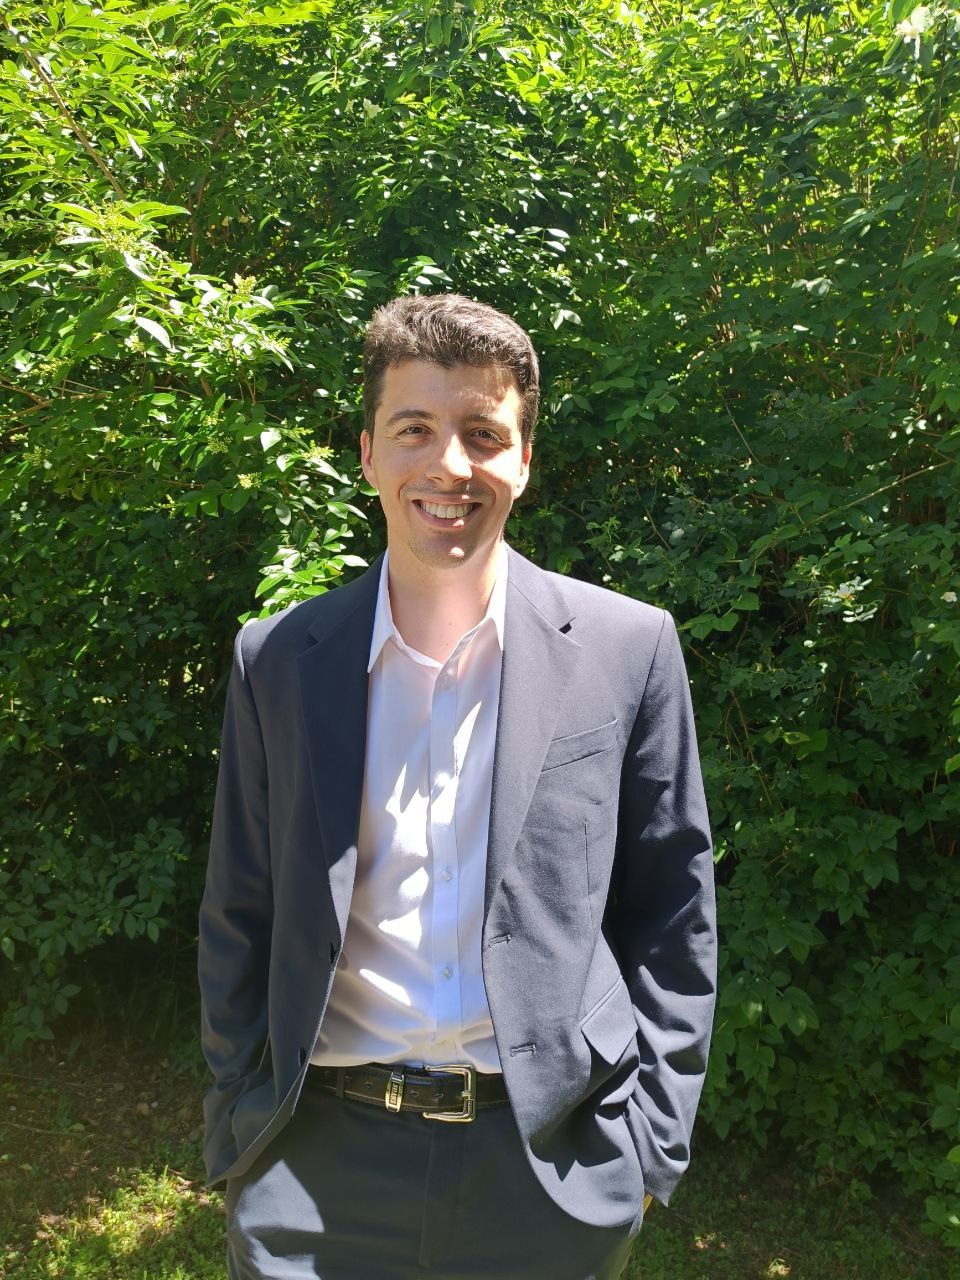
\includegraphics[scale=.18]{../risorse/foto.jpg}}
    \end{tikzpicture}
\end{figure}


\vspace{1.5mm}
{\large Dati personali e recapiti}

\vspace{2.2mm}
\faBaby \quad Nato il 11/09/2000 a Segrate (MI)

\vspace{2.2mm}
\begin{tabular}{@{}l@{\quad}p{0.8\textwidth}}
   \faMapMarker & Residente a \\
                & Bellinzago Lombardo (MI), \\
                & via Lombardia 19, 20060 \\
\end{tabular}
\vspace{1.5mm}

\faPhone \quad +39 3664181411

\faEnvelope \quad \href{mailto://gchirico28@gmail.com}{gchirico28@gmail.com}

\rule{\linewidth}{0.4pt}

{\large Link}

\faLinkedin \quad \href{https://tinyurl.com/gchirlinkedin}{https://tinyurl.com/gchirlinkedin}

\faGithub \quad \href{https://github.com/giorgio-hash}{github.com/giorgio-hash}

\rule{\linewidth}{0.4pt}

{\large Soft skills}

\faCircleNotch \quad teamworking

\faCircleNotch \quad problem solving

\faCircleNotch \quad capacità di analisi

\rule{\linewidth}{0.4pt}

{\large Lingue}

\faLanguage \quad Inglese  (B2)

\faLanguage \quad Tedesco  (A2)

\faLanguage \quad Spagnolo (A1)

\rule{\linewidth}{0.4pt}

{\large Hobby}

\faLock \quad Conferenze InfoSec

\faCloud \quad TryHackMe (lvl.8)

\faFish \quad acquariofilia

\faLeaf \quad giardinaggio

\rule{\linewidth}{0.4pt}

{\large Badge e attestati}

\faAward \quad Completato Advent Of Cyber 2024 
\href{https://tinyurl.com/THM-fundamentCert}{https://tinyurl.com/THM-fundamentCert}

\end{minipage}
\hfill
\begin{minipage}[t]{0.65\textwidth}
\setlength{\baselineskip}{1.4\baselineskip}

{\tiny Autorizzo il trattamento dei dati personali presenti nel CV ai sensi del D.lgs.2018/101 e del GDPR (Regolamento UE 2016/2019)}
\vspace{0.3cm}


{\huge Giorgio Chirico}

{\large Dottore in Ingegneria Informatica (classe L-08)}

\vspace{0.5cm}
 
Dottore in ingegneria informatica, specializzato nello sviluppo e verifica di sistemi in rete. Ho conoscenze in Big Data, AI, Machine Learning e passione per tematiche di sicurezza digitale quali Offensive Security, Security-By-Design e protezione dati.


\vspace{0.15cm}

\makeatletter
\newcommand{\FormazioneBox}{%
    \begin{tikzpicture}[remember picture,overlay]
        \coordinate (boxtop) at ($(current page.north west)+(20pt+0.5cm,-\dimexpr\pagetotal+1.5\baselineskip\relax)$);
        \node[anchor=north west, draw={rgb,255:red,18;green,44;blue,71}, fill={rgb,255:red,18;green,44;blue,71}, text=white, rounded corners, inner sep=6pt, minimum width=\dimexpr\paperwidth-40pt-0.5cm\relax] at (boxtop) {%
            \begin{minipage}[t]{\dimexpr\paperwidth-40pt-0.5cm-12pt\relax}%
                {\large \color{white}Formazione}\color{white}\rule{\linewidth}{0.4pt}
            \end{minipage}%
        };
    \end{tikzpicture}%
}
\makeatother

\FormazioneBox

\vspace{0.8 cm}

{\large \textbf{Laurea Magistrale in Ingegneria Informatica}}

{\small Università di Bergamo, Dalmine (BG)}
\begin{itemize}
    \item Settembre 2023 - oggi
    \item Frequentante full-time. Specializzazione in Sistemi In Rete
\item Competenze nel mondo dei \textbf{dati}, sistemi di integrazione, ontologie, framework per i big data. Concetti di anonimizzazione, privacy e principali vulnerabilità.
\item Competenze con \textbf{modelli} in area AI, Machine Learning e ricerca operativa. Conoscenze in modelli di automazione. 
\item Competenze di \textbf{programmazione avanzata} con ottimizzazione degli algoritmi, uso di design pattern, debug ed analisi della memoria, uso di regex e realizzazione di compilatori, applicazione delle tecniche formali di testing e verifica del software.
\item Conoscenze in teoria della \textbf{trasmissione} codificata, sensoristica e comunicazione wireless su reti estese.
\item Conoscenze in \textbf{crittografia}, hashing, firma e principali \textbf{vulnerabilità} dei sistemi.\end{itemize}
{\large \textbf{Laurea Triennale in Ingegneria Informatica} }

{\small Università di Bergamo, Dalmine (BG)}
\begin{itemize}
    \item Settembre 2019 - Settembre 2023.
\item Formazione di base per l'ingegneria, \textbf{ingegneria del software} e \textbf{reti telcom}. 
\item Tesi a tema \textbf{Offensive Security}: \href{https://github.com/giorgio-hash/tesi-triennio}{"Vulnerabilità Di Fuga Da Docker"}
 \end{itemize}

{\large \textbf{Diploma Tecnico Perito Informatico}}

{\small Istituto Guglielmo Marconi, Gorgonzola (MI)}
\begin{itemize}
    \item Settembre 2014 - Giugno 2019
    \item Basi di \textbf{gestione dati strutturati e non}, programmazione procedurale ed OOP, programmazione web, \textbf{infrastrutture web sicure} per servire contenuti.
\end{itemize}

\vspace{0.15cm}

\makeatletter
\newcommand{\EsperienzaBox}{%
    \begin{tikzpicture}[remember picture,overlay]
        \coordinate (boxtop) at ($(current page.north west)+(20pt+0.5cm,-\dimexpr\pagetotal+1.5\baselineskip\relax)$);
        \node[anchor=north west, draw={rgb,255:red,18;green,44;blue,71}, fill={rgb,255:red,18;green,44;blue,71}, text=white, rounded corners, inner sep=6pt, minimum width=\dimexpr\paperwidth-40pt-0.5cm\relax] at (boxtop) {%
            \begin{minipage}[t]{\dimexpr\paperwidth-40pt-0.5cm-12pt\relax}%
                {\large \color{white}Esperienza Lavorativa}\color{white}\rule{\linewidth}{0.4pt}
            \end{minipage}%
        };
    \end{tikzpicture}%
}
\makeatother

\EsperienzaBox

\vspace{0.8 cm}

{\large \textbf{Programmatore Java, Scuola Lavoro}}

{\small  Azienda IT consulting \textit{Open Gate}, Gorgonzola (MI)}

\begin{itemize}
    \item Giugno 2017 - Luglio 2017
    \item Lavoro di gruppo per produrre un videogioco 2D in Java, dotato di GUI
\end{itemize}

{\large \textbf{Lezioni private, autonomo}}

{\small In remoto e a domicilio}

\begin{itemize}
    \item 2020 - oggi
    \item Aiuto i ragazzi delle superiori/università nello studio e nel loro orientamento.
\end{itemize}

\end{minipage}

\end{document}
